\documentclass[twocolumn]{article}

\newcommand{\authorname}{Austin Jetrin Maddison}
\newcommand{\course}{Discrete Simulation}
\newcommand{\courseid}{ICMA393}
\newcommand{\docname}{HW2}
\newcommand{\titletext}{\course: \docname}

%\usepackage{fontspec}	
\usepackage[no-math]{fontspec}	
\setmainfont{HelveticaNowText}
\newfontface\hh{HelveticaNowText-ExtraBold}
\newfontface\lt{HelveticaNowText-Light}      
\newfontface\xx{HelveticaNowText-ExtraLight} 
\newfontface\mm{HelveticaNowText Medium}

\newfontfamily{\displayfont}{HelveticaNowDisplay}
\newfontface\dslt{HelveticaNowDisplay-Light}
\newfontface\dsmm{HelveticaNowDisplay-Medium}
\newfontface\dsbd{HelveticaNowDisplay-Bold}

\newfontfamily{\microfont}{HelveticaNowMicro}
\newfontface\mclt{HelveticaNowMicro-Light}
\newfontface\mcmm{HelveticaNowMicro-Medium}
\newfontface\mcbd{HelveticaNowMicro-Bold}

\setmonofont{SFMono}

\usepackage[lining]{FiraSans}
\usepackage[fakebold]{firamath-otf}
\usepackage{unicode-math}
\setmathfont{FiraMath}
\renewcommand*\oldstylenums[1]{{\firaoldstyle #1}}


\usepackage{microtype}   % Improves text appearance with microtypography
\usepackage{amsmath}     % For better math support
\usepackage{graphicx}    % For including graphics
\usepackage{lipsum}      % For placeholder text
\usepackage{enumitem}
\usepackage{xcolor}
\usepackage{svg}
\usepackage{svg-extract}
\usepackage{caption}
\usepackage{float}


\usepackage[a4paper, margin=0.8in, columnsep=20pt]{geometry}

\captionsetup{font=small}
\definecolor{gray}{rgb}{0.55, 0.55, 0.55}
\setlength{\columnsep}{20pt}  % Space between columns

% Headers and Footers
\usepackage{fancyhdr}
\pagestyle{fancy}
\fancyhf{}

% First Page
\fancypagestyle{plain}{
\fancyfoot[R]{\small \thepage} 
\fancyfoot[L]{} 
\fancyhead[L]{}
\fancyhead[R]{}
}

% Custom header
\fancyfoot[L]{\scriptsize \MakeUppercase{ \microfont \courseid~\course}}
\fancyhead[L]{\scriptsize \MakeUppercase{ \microfont \docname}}
\renewcommand{\headrulewidth}{0pt}

% Custom footer
%\fancyfoot[L]{\small Title, Date}
\fancyfoot[R]{\small \thepage}

% Line spacing
\usepackage{setspace}
\setstretch{1.15}  % Slightly more space between lines

%\setlength{\mathindent}{0pt} % This removes the indentation for equations

% Section formatting
\usepackage{titlesec}
\titleformat{\section}[block]{\large\dsbd}{\thesection.}{1em}{}
\titleformat{\subsection}[block]{\normalsize \mm}{\thesubsection.}{1em}{}

% Bibliography style
\usepackage[numbers,sort&compress]{natbib} % For numbered citations

% Hyperlinks
\usepackage{hyperref}
\hypersetup{
    colorlinks=false,
    linkcolor=blue,
    citecolor=blue,
    urlcolor=blue,
    pdftitle={Research Paper Title},
    pdfauthor={Author's Name},
}

\usepackage{listings}
\lstset{
  language=Python,                     % Use Python language syntax
  basicstyle=\ttfamily\footnotesize,           % Use modern monospace font for code
  keywordstyle=\bfseries\color{black},   % Bold and blue keywords
  stringstyle=\color{black},              % Strings in red
  commentstyle=\color{gray},            % Comments in gray
  showstringspaces=false,               % Don't show spaces in strings
  breaklines=true,                      % Break long lines
  tabsize=4,                            % Set tab size to 4 spaces
}


\begin{document}
\fontsize{9.5}{11.5}\selectfont % Set font size to 12pt with a baseline of 14pt

% Title 
\title{
  \raggedright
  \Large \displayfont \strong{\courseid~\titletext} \\[5pt]  % Adjust spacing if needed
%  \raggedleft
  \small Mahidol University International College \\
  \small \authorname \\ 
  \small \today
}
\date{} 

%
\twocolumn[{
	\vspace*{-1cm}
	\maketitle
	\vspace*{-0.5cm}
}]

\section{Birthday Problem}\label{p1}


\begin{figure}
	\centering
	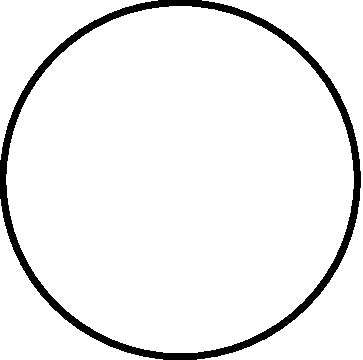
\includegraphics[width=0.7\linewidth]{../drawings/p1_1}
	\caption{}
	\label{fig:path1}
\end{figure}

\begin{figure}
	\centering
	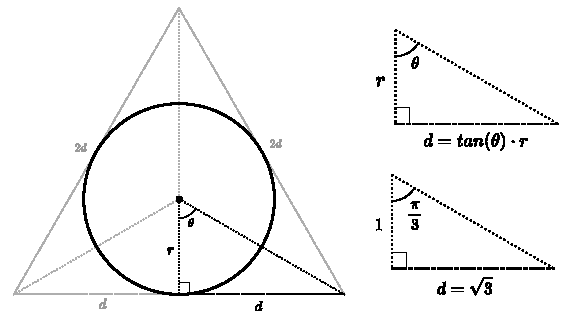
\includegraphics[width=0.7\linewidth]{../drawings/p1_2}
	\caption{}
	\label{fig:path2}
\end{figure}

\begin{figure}
	\centering
	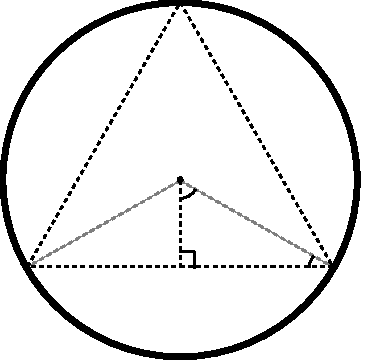
\includegraphics[width=0.7\linewidth]{../drawings/p1_3}
	\caption{}
	\label{fig:path3}
\end{figure}

\begin{figure}
	\centering
	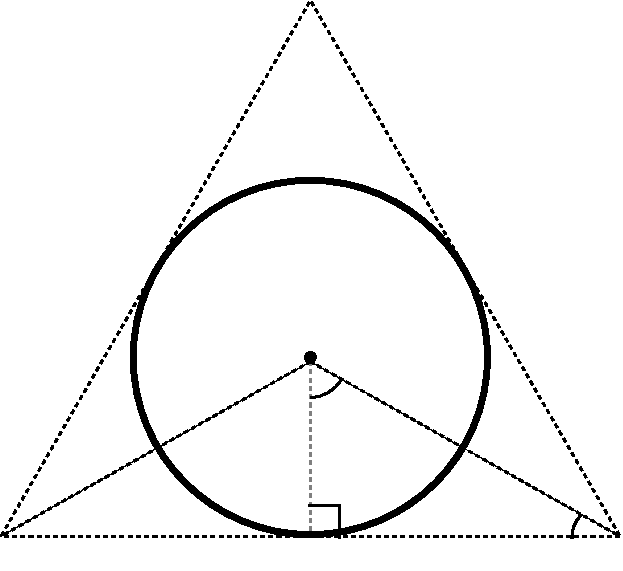
\includegraphics[width=0.7\linewidth]{../drawings/p1_4}
	\caption{}
	\label{fig:path4}
\end{figure}






The simulations ran were set to $seed=27$ \\and $N=400000$.

\begin{enumerate}[label=\alph*),itemsep=-1.5em]
    
\item 
\begin{align*}
p_{10} &= 0.11686 \\
CI &= [0.11685, 0.11885]
\end{align*}


\item 
\begin{align*}
p_{20} &=  0.41126 \\
CI &= [0.41125, 0.41430]
\end{align*}


\item
\begin{align*}
p_{30} &= 0.70595 \\
CI &= [0.70594, 0.70877]\\
\end{align*}

\item 
Found $n$ that satisfies the condition $p_n \ge 0.5$ from running the simulation on a range of $n$'s $[0, 50]$ and selecting the first $p_n \ge 0.5$.

\vspace{-5pt}
\begin{figure}[H]
    \centering
    \includesvg[width=0.5\textwidth]{p1_d.svg} % Adjust the width as needed
    \caption{The first point $\geq p=0.5$ was $p_{23}=0.506$ which satisfies the condition.}
\end{figure}




\item 
We can model $p_n$ using a product function. We do this by getting the product of probabilities where we always pick somebody with a unique birthday. Then we invert the result by minus 1 to get the probability of picking somebody with a non-unique birthday.

\vspace{-10pt}
\begin{align*}
p(n) = 1 - \prod_{i=0}^{n} \frac{\text{365} - i}{365}
\end{align*}
\vspace{-10pt}

\begin{figure}[H]
    \centering
    \includesvg[width=0.5\textwidth]{p1_e.svg} % Adjust the width as needed
    \caption{$p(n)$ results are similar to the simulation. The difference between simulation $p_n$ and $p(n)$ is $MSE = 2.013\times10^{-7}$.}
\end{figure}
\vspace{-14pt}
For all intensive purposes $p(n)$ models the results in simulation $p_n$. 

\end{enumerate}


\section{Alice and Bob Play a Game}
The strategy I let Alice have is the following...
\\

\noindent
\textbf{Case 1: Found Exclusive Output}\\
She presses the button recording $n$ output values $x_1, x_2, ... x_n$.
As she records each output she checks whether $x_i$ is exclusive to one of the buttons output range. If $x_i$ is exclusive she returns the corresponding button as the answer.
\\

\noindent
\textbf{Case 2: No Exclusive Output}\\
If she presses the button $n$ times with no exclusive output appearing. She calculates $\bar{x}$ and finds the minimum difference between the mean output range of the 2 buttons. She returns the corresponding button that gets the minimum distance.
\\

\noindent
\textbf{Find $n$ such that Alice is correct $\ge 0.99$}
I sampled Alice's strategy varying $n$ between $[0, 500]$ and extracted the first n that results in probability atleast $0.99$. I set the $seed=27$ and  ran $400000$ trials for all $n$'s.

\begin{figure}[H]
	\centering
	\includesvg[width=0.5\textwidth]{p2_1.svg} % Adjust the width as needed
	\caption{The first point to $\ge p=0.99$ was $p_{384}=0.990$ which satisfies the condition.}
	\label{fig:Figure2}
\end{figure}

\begin{figure}[H]
	\centering
	\includesvg[width=0.5\textwidth]{p2_2.svg} % Adjust the width as needed
	\caption{Crop of Figure~\ref{fig:Figure2}.}
\end{figure}

\noindent
\textbf{Psuedocode}\\
Although the source code differs because loops are removed for speed, the idea is the same.


\begin{lstlisting}
xs = []
for i in range(0, n):	
	x_n = button_unknown.get_next_value()
	xs.append(x_n) 	
	
	# Case 1: Found exclusive output.
	if(x_n == 1)
		return 1  # it is button 1
	if(x_n == 100)
		return 2  # it is button 2
		
# Case 2: No exclusive output. Evaluate the minimum distance of means.
x_mean = sum(xs) / n
button_1_mean = (1 + 99)/2
button_2_mean = (2 + 100)/2

return argmin([abs(x_mean - button_1_mean), abs(x_mean - button_2_mean)]) + 1
\end{lstlisting}



\raggedbottom
\section{Practice with Uniform and Geometric Distributions}

First find E[X] and V[X] of the geometric distribution. Since X is a fair dice $p\{X=5\}= 1/6$.

\vspace{-10pt}
\begin{align*}
E[X] &= \frac{1}{1/6} = 6 \\
V[X] &= \frac{1-1/6}{(1/6)^2} = 30 \\
\end{align*}

\vspace{-20pt}
Then I do the same for uniform distribution of $Y$ while equating the corresponding known values from $X$.

\vspace{-25pt}
\begin{align*}
E[Y] &= \frac{n-1}{2} = 6 \\
V[Y] &= \frac{(n^2-1)}{12} = 30 \\
\end{align*}

\vspace{-18pt}
Since $n$ is determined by the setting of $a$ and $b$ we can rewrite it like this.

\vspace{-10pt}
\begin{align*}
E[Y] &= \frac{(b-a+1)-1}{2} = 6 \\
V[Y] &= \frac{(b-a+1)^2-1}{12} = 30 \\
\end{align*}

\vspace{-20pt}
Now it's easy to find $a$ and $b$ by solving the system of equations. However I am not going to do that because that is not how I found it at first. \\
\vspace{-10pt}
\\
What I did is rearranged $E[Y]$ such that $a+b=12$. Then I did a search of pairs of $a,b$ st, $a+b=12$ and $a<b$ until I got $V[Y]=30$.  


\vspace{-10pt}
\begin{figure}[H]
    \centering
    \includesvg[width=0.5\textwidth]{p3.svg} % Adjust the width as needed
    \vspace{-10pt}
    \caption{The size and opacity of the discs is the inverse distance away from $V[Y] = 30$.}
\end{figure}

\vspace{-10pt}
For $E[X]=E[Y]$ and $V[X]=V[Y]$,
\vspace{-10pt}
\begin{align*}
a=-3, b=15
\end{align*}


\section*{Source Code}
\href{https://github.com/AustinMaddison/discrete-simulation/tree/main/hw1/source}{https://github.com/AustinMaddison/discrete-simulation/tree/main\docname/source}

% References
%\bibliographystyle{unsrt}
%\bibliography{references}

\end{document}
